\section{Current Work in Progress}
	\scriptsize
    \begin{frame}{Wave Propagation and Error Analysis}
    	\scriptsize
    	\textbf{Wave propagation parameters (LeVeque et al.):}
    	The scheme can be characterized by three integers $(m_1, m_2, m_3)$:
    	\begin{itemize}
    		\item $m_1$: Correction wave (1 = not included, 2 = included)
    		\item $m_2$: Transverse propagation (0 = none, 1 = increment only, 2 = increment + correction)
    		\item $m_3$: Double-transverse propagation (0 = none, 1 = increment only, 2 = increment + correction)
    	\end{itemize}
    	
    	\medskip
    	\textbf{Error computation:}  
    	On a coarse grid, define
    	\[
    	E(h) = U(h) - U(h/2), \quad
    	E(h/2) = U(h/2) - U(h/4)
    	\]
    \end{frame}
    
    %-------------------------------------------------------
    
    \begin{frame}{Accuracy Analysis}
    	\scriptsize
    	Consider approximations of the three-dimensional hyperbolic
    	system
    	\begin{align}
    		    	\partial_tQ + AQ_x + BQ_y + CQ_z = (D(wx, wy,wz) + DrE)Q \label{3D-hyperbolic}
    	\end{align}
        with externally imposed velocity gradient $w_x=1=w_y$ and $w_z=0$.
 
    	% Initialwert direkt über der Tabelle
    	Let 
    	\[
    	r = \sqrt{(x-40)^2+(y-30)^2+(z-50)^2}, \quad
    	c^0_0(x, y, k, 0) = \exp(-0.01 \, r^2)
    	\] 
    	be the initial value.
    	
    	\medskip
    	\centering
    	\begin{tabular}{|c|c|c|c|c|c|c|c|}
    		\hline
    		Method & Grid & \multicolumn{2}{c|}{N=1} & \multicolumn{2}{c|}{N=2} & \multicolumn{2}{c|}{N=7} \\
    		\cline{3-8}
    		&  & $L_1$ Error & EOC & $L_1$ Error & EOC & $L_1$ Error & EOC \\
    		\hline
    		(1,1,1) & 32  & $5.57\cdot10^{-4}$ & -    & $5.47\cdot10^{-4}$ & -    & $5.01 \cdot10^{-4} $ & - \\
    		& 64  & $3.54\cdot10^{-4}$ & 0.65 & $3.40\cdot10^{-4}$ & 0.68 & $2.93\cdot10^{-4}$ & $0.77$ \\
    		& 128 & $1.79\cdot10^{-4}$ & 0.98 & $1.80\cdot10^{-4}$ & 0.91 & - & - \\
    		\hline
    		(2,2,2) & 32  & $1.79\cdot10^{-4}$ & -    & $2.00\cdot10^{-4}$ & -    & $1.83\cdot10^{-4}$ & - \\
    		& 64  & $4.66\cdot10^{-5}$ & 1.94 & $5.45\cdot10^{-5}$ & 1.86 & $4.82\cdot10^{-5}$ & 1.92 \\
    		& 128 & $1.17\cdot10^{-5}$ & 1.99 & $1.38\cdot10^{-5}$ & 1.98 & - & - \\
    		\hline
    	\end{tabular}
    
    	\vspace{0.5em}
    	\footnotesize{
    		\textbf{Table:} Accuracy analysis for the component $c^0_0$ of (\ref{3D-hyperbolic}) using $D_r=1$. The time step was limited by the CFL condition, with $cfl \le 0.45$ for method (1,1,1) and $cfl \le 0.9$ for method (2,2,2).  
    	}
    \end{frame}
    
    
    %-------------------------------------------------------
    %Example 1
    %-------------------------------------------------------
    %if (xi .lt. 50.d0) then
    % uzk = 10.0d0
    %else
    % uzk = -10.0d0
    % end if
    % uxi = 0.d0
    % uyi = 0.d0
    % call defineAllgMatrixN1_driftdiffusion(A, Dr, uxi,
    %  &           uyi, uzk, 0.d0, 0.d0, 0.d0, 0, 0, 0, 0.d0)
    
    % qinit
    %  r1 = dsqrt((xi-40.d0)**2+(yj-50.d0)**2+(zk-50.d0)**2)
    %  r2 = dsqrt((xi-60.d0)**2+(yj-50.d0)**2+(zk-50.d0)**2)
    %  q(i,j,k,1) = exp(-0.01*r1**2) + exp(-0.01*r2**2) 
    %-------------------------------------------------------
    

    %-------------------------------------------------------
    %Example 2
    %-------------------------------------------------------
    %  if (xi .le. 50.d0) then
    %  wxi = 1.d0
    %  wyj = 1.d0
    %  wzk = 0.d0
    %    else
    %  wxi = -1.d0
    %  wyj = -1.d0
    %  wzk = 0.d0
    %  end if
    %  r1 = dsqrt((xi-40.d0)**2+(yj-50.d0)**2+(zk-50.d0)**2)
    %  r2 = dsqrt((xi-60.d0)**2+(yj-50.d0)**2+(zk-50.d0)**2)
    %  q(i,j,k,1) = exp(-0.01*r1**2) + exp(-0.01*r2**2) 
    %-------------------------------------------------------
     \begin{frame}{Example 1}
    	\scriptsize
    	\begin{figure}[H]
    		\centering
    		\begin{minipage}{0.4\textwidth}
    			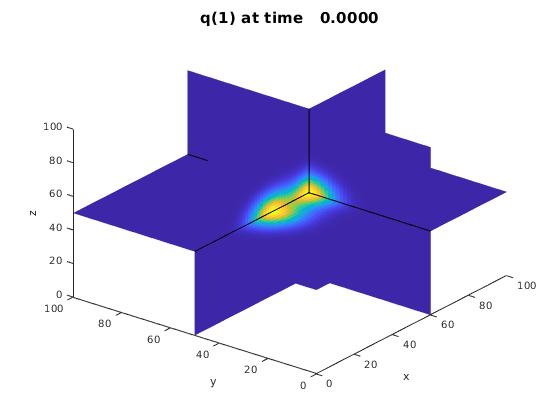
\includegraphics[scale=0.21]{Bilder_3D/2Glocken_wxi_wyj_wzi_2Cluster_t=0}
    		\end{minipage}
    		\hfill 
    		\begin{minipage}{0.4\textwidth}
    			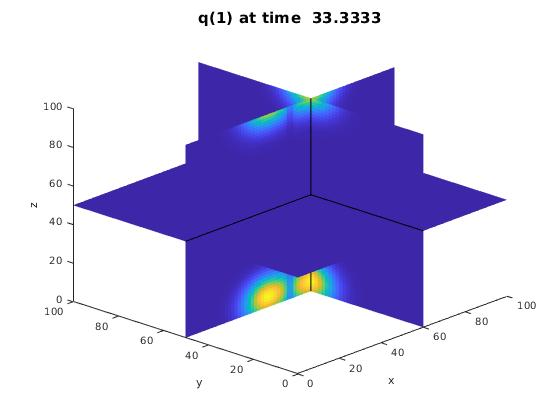
\includegraphics[scale=0.21]{Bilder_3D/2Glocken_wxi_wyj_wzi_2Cluster_t=33}
    		\end{minipage}
    	\end{figure}
    	\begin{figure}[H]
    		\centering
    		\begin{minipage}{0.4\textwidth}
    			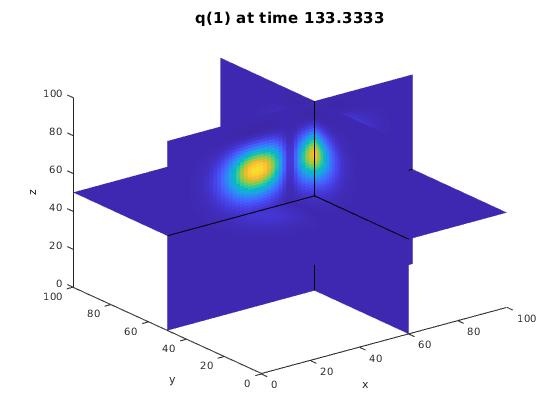
\includegraphics[scale=0.21]{Bilder_3D/2Glocken_wxi_wyj_wzi_2Cluster_t=133}
    		\end{minipage}
    		\hfill 
    		\begin{minipage}{0.4\textwidth}
    			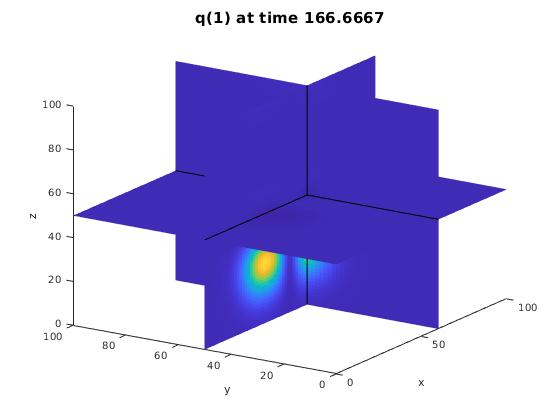
\includegraphics[scale=0.21]{Bilder_3D/2Glocken_wxi_wyj_wzi_2Cluster_t=166}
    		\end{minipage}
    		\caption{Evolution of $c^0_0$ at different times, showing two Gaussian clusters transported in opposite directions by a piecewise constant velocity field ($w_x=w_y=1$ for $x<50$, $w_x=w_y=-1$ otherwise, and $w_z=0$ everywhere).}
    	\end{figure}
    \end{frame}
    
    \begin{frame}{Conclusion}
 content
    \end{frame}

